\subsection{Additional Embodiment: WX200}\label{sec:wx200}
An ongoing experiment applies the pipeline to the five-DoF WX200 serial manipulator. This setting changes the robot mechanism while retaining the skill-learning and composition schedule. Figure~\ref{fig:wx200} reserves the setup and rollout illustrations. Quantitative success rates will be added after the evaluation is complete.

\begin{figure*}[!t]
\centering
\IfFileExists{figures/wx200/panel.pdf}{\includegraphics[width=\textwidth]{figures/wx200/panel.pdf}}{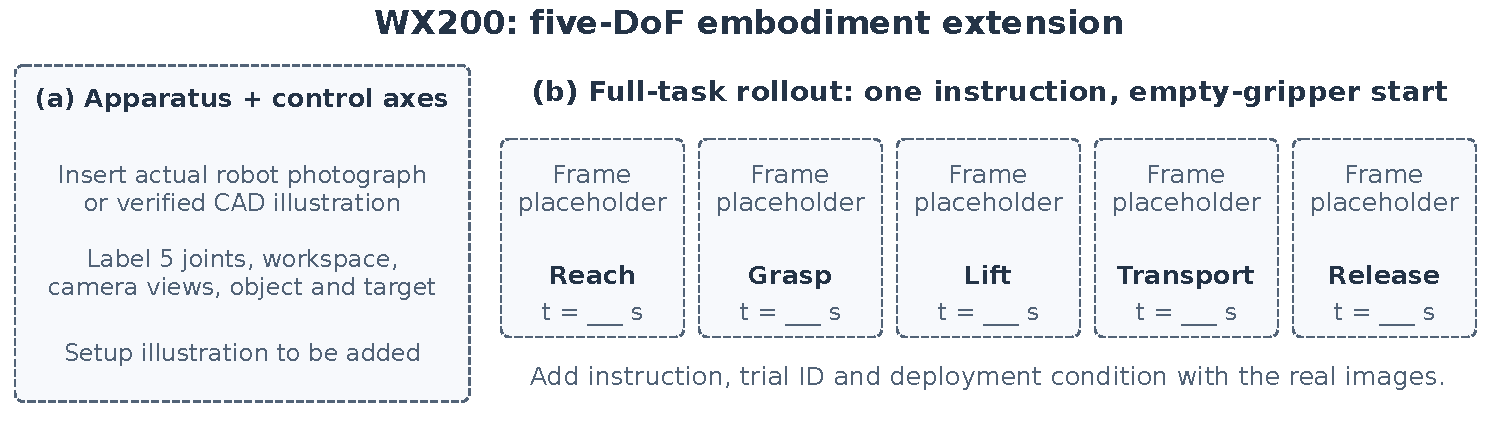
\includegraphics[width=\textwidth]{figures/wx200_slots.pdf}}
\caption{WX200 evaluation layout. (a) Apparatus, workspace, cameras, and control axes. (b) Reach, grasp, lift, transport, and release under one instruction. The current panels reserve space for setup images and timestamped rollout frames from the ongoing experiment.}
\label{fig:wx200}
\end{figure*}
